\begin{figure}[!h]
	\centering
	\subbottom[\label{fig:mspascal1}]{
		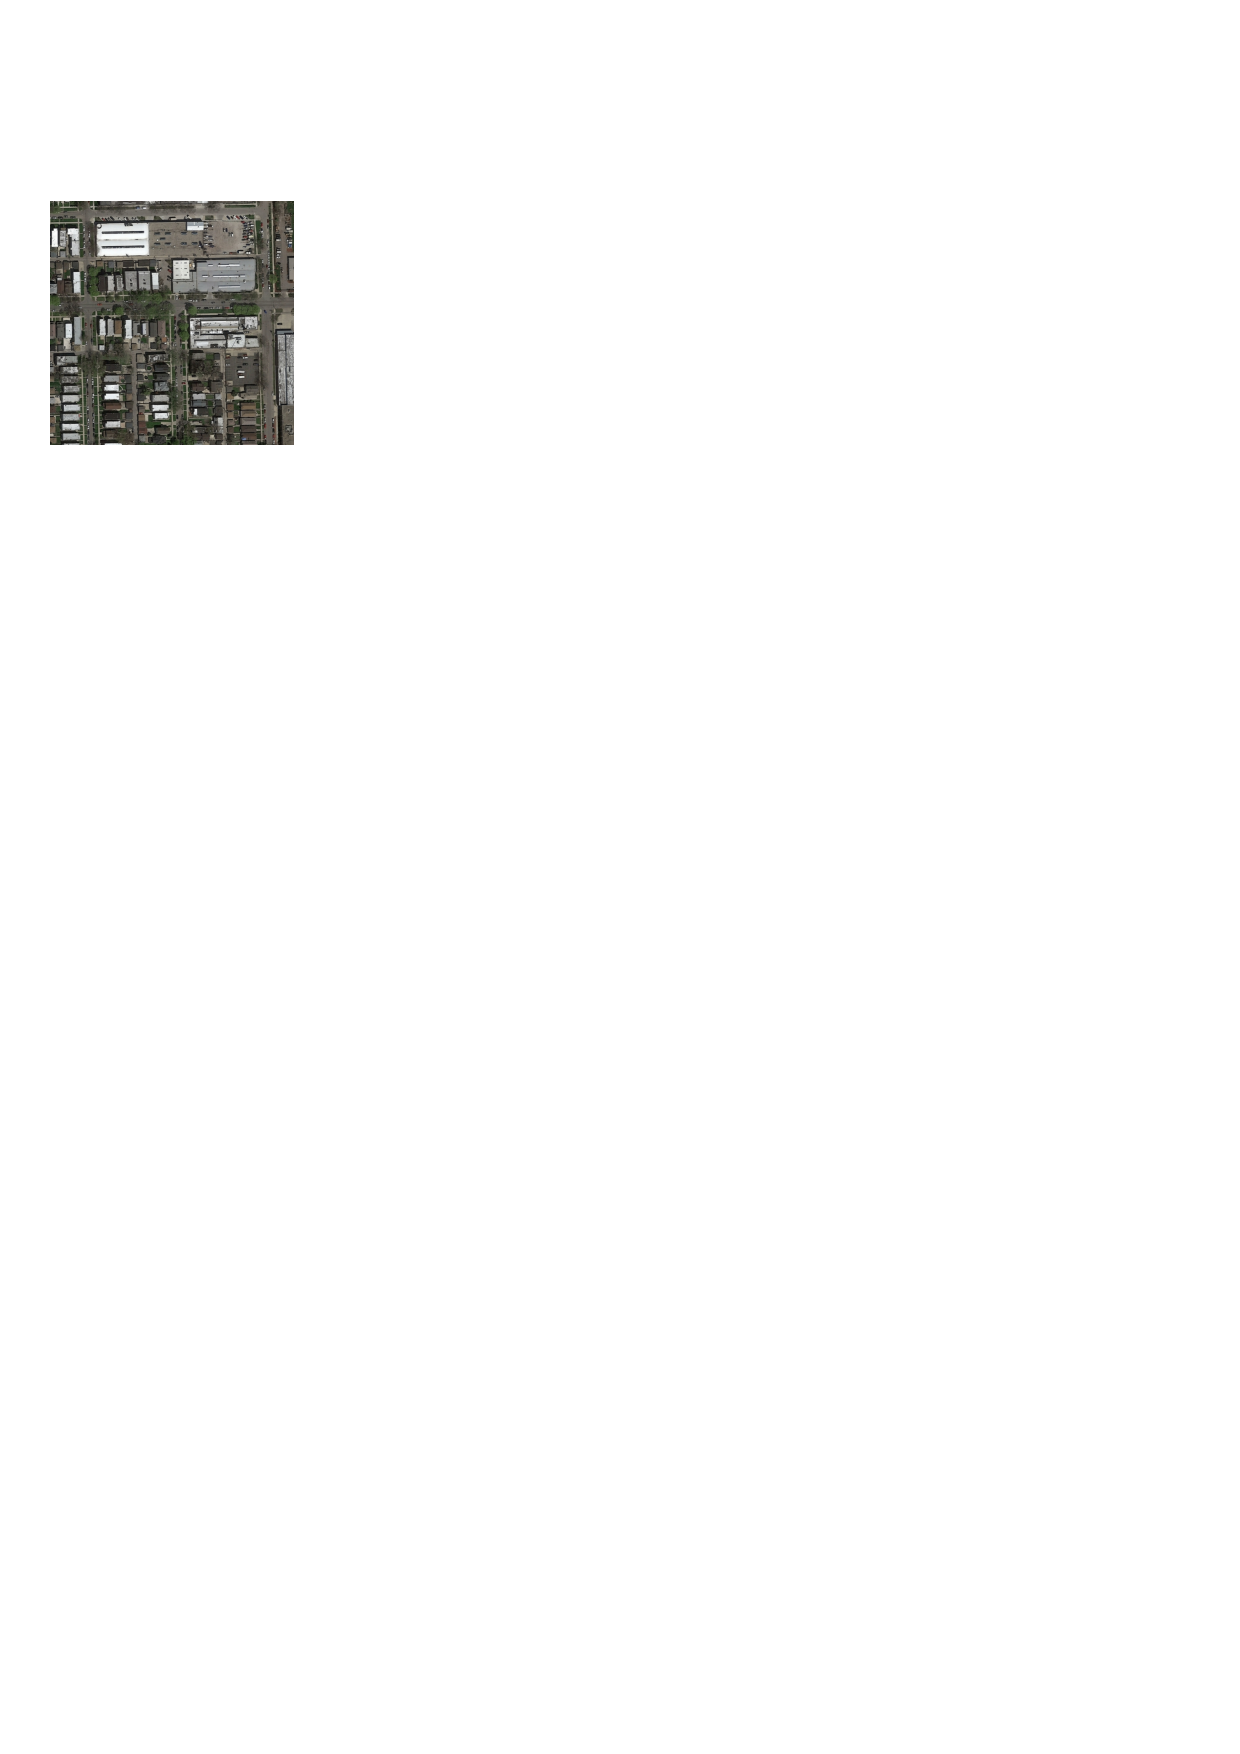
\includegraphics[width=\figfigfigfig\textwidth]{2-00-0.pdf}
	}
	\subbottom[\label{fig:mspascal2}]{
		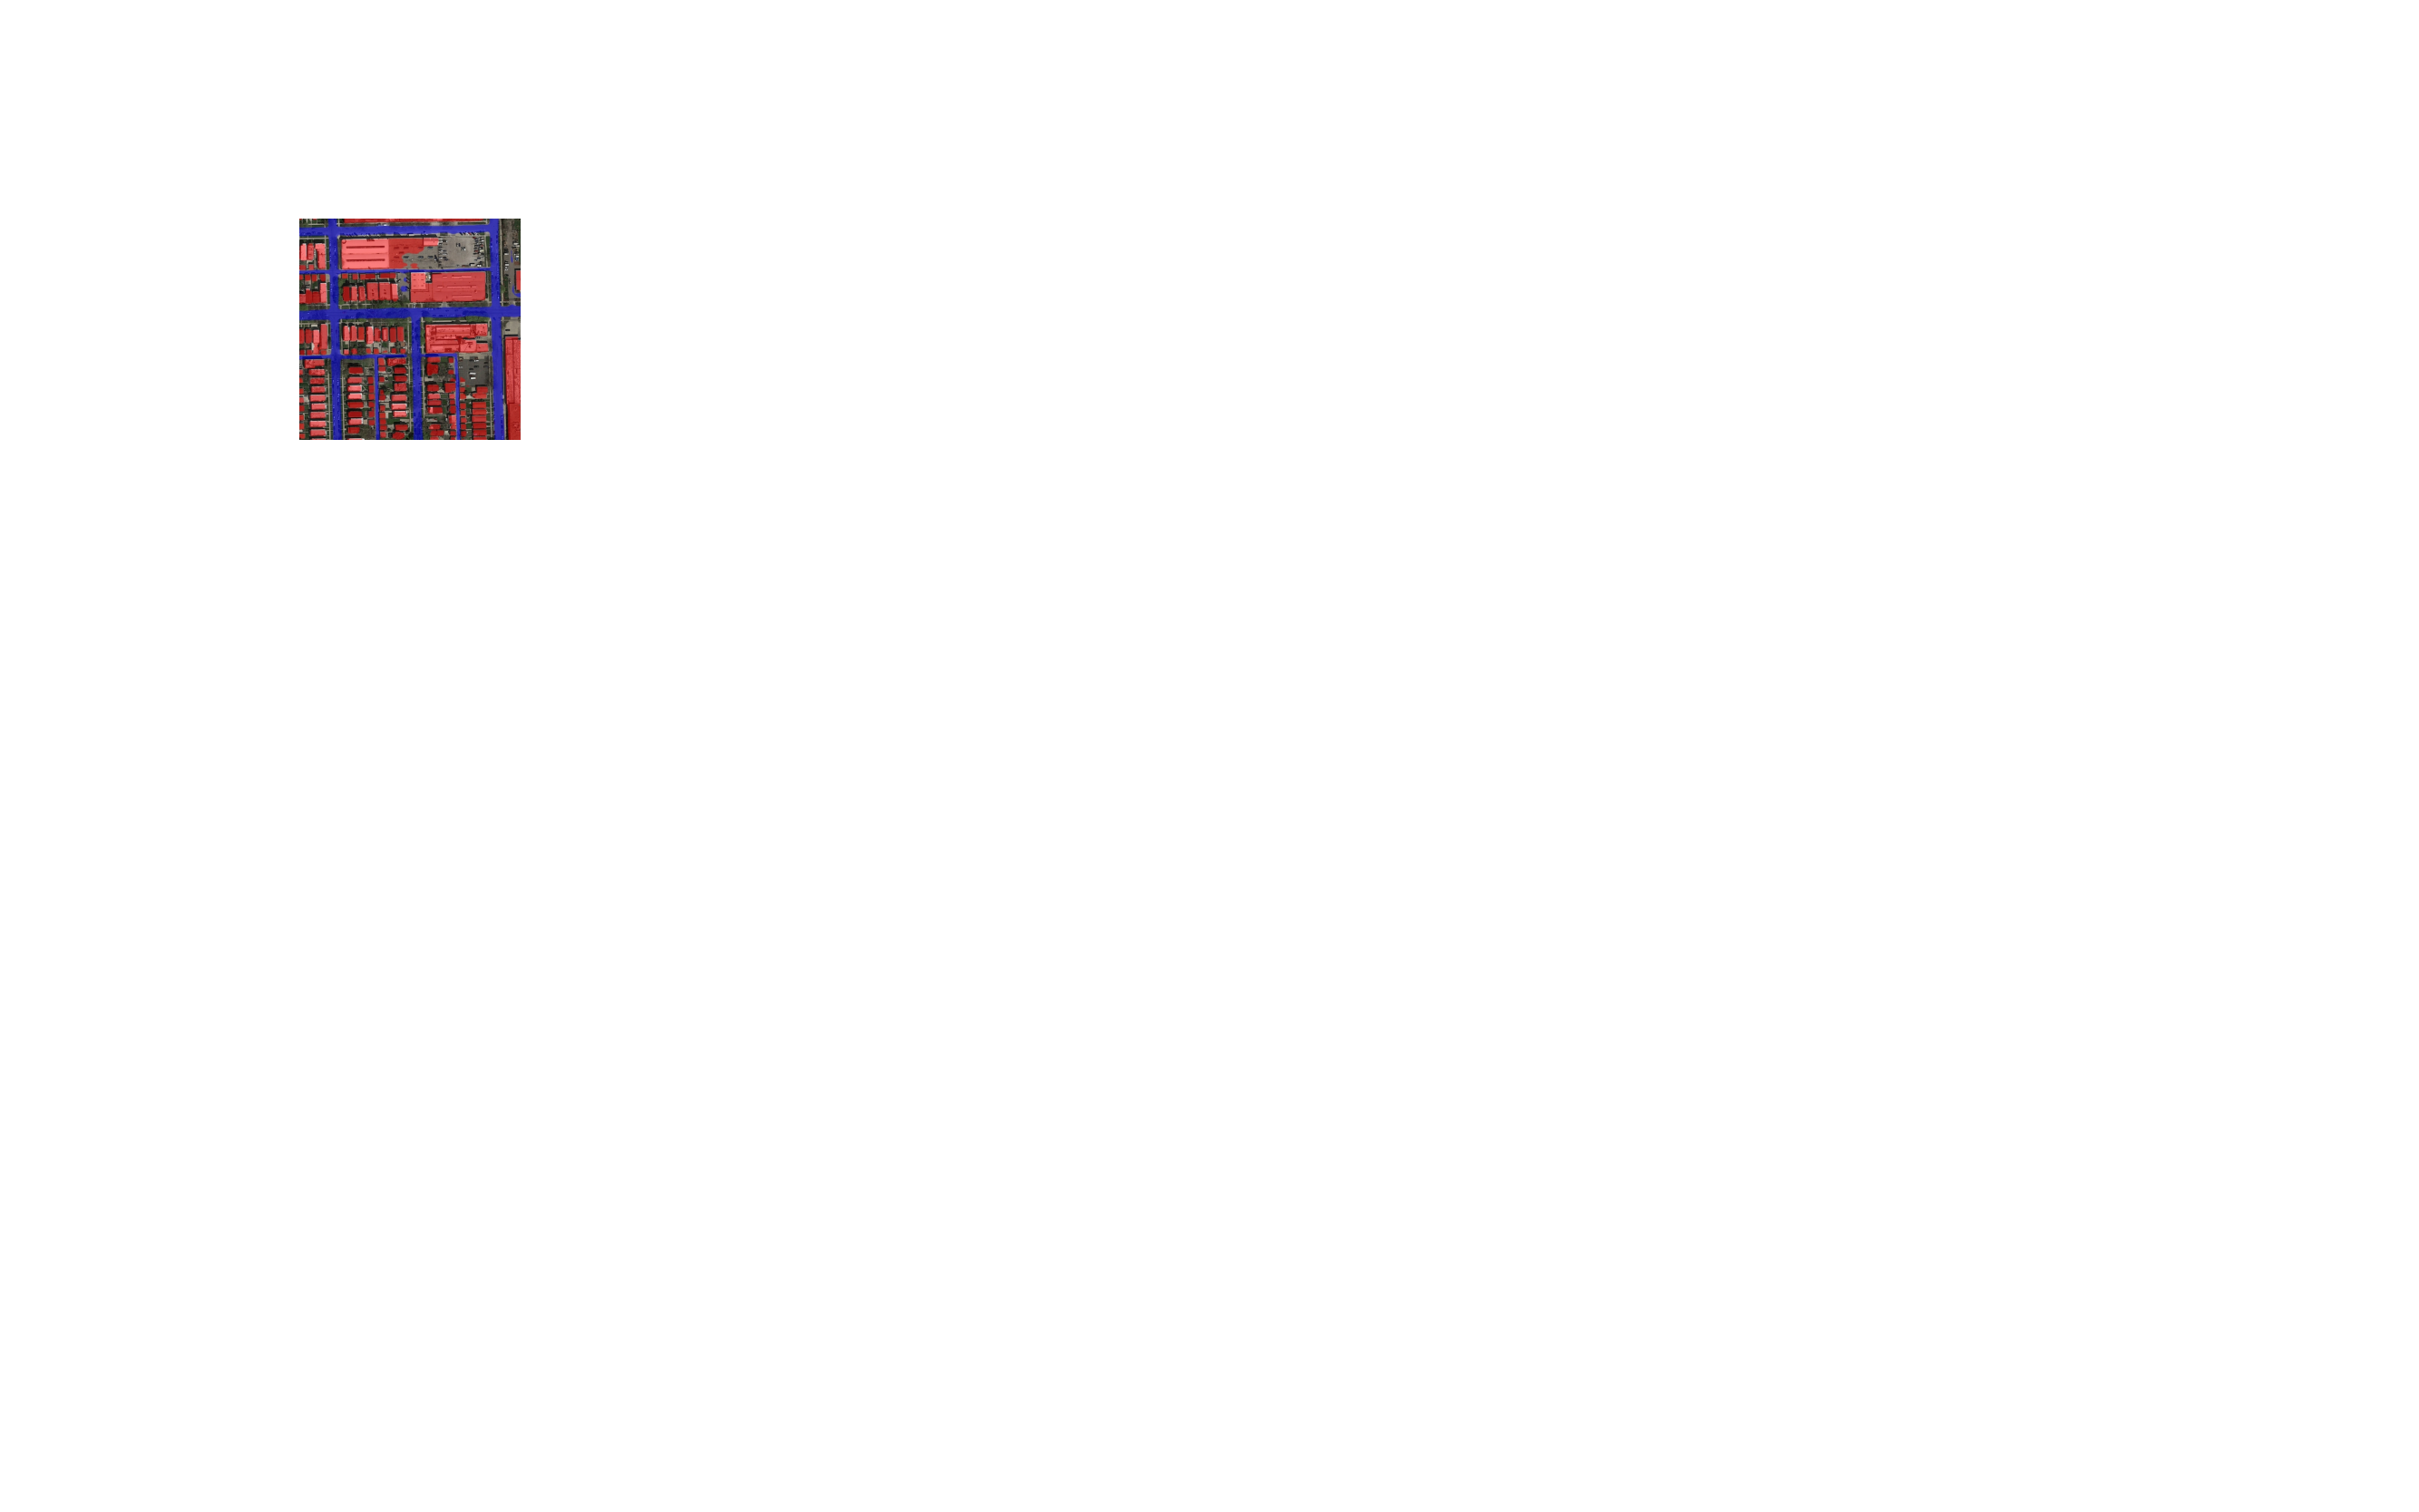
\includegraphics[width=\figfigfigfig\textwidth]{2-00-1.pdf}
	}
	\subbottom[\label{fig:mspascal3}]{
		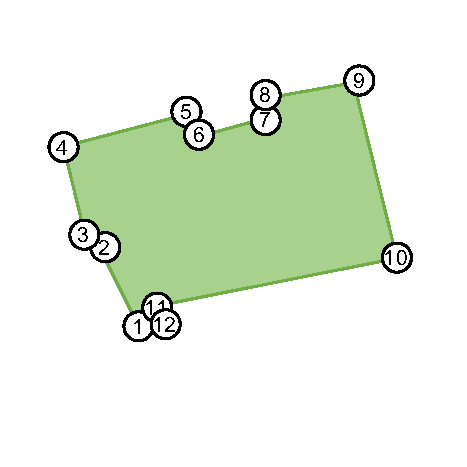
\includegraphics[width=\figfigfigfig\textwidth]{2-00-2.pdf}
	}
	\subbottom[\label{fig:mspascal4}]{
		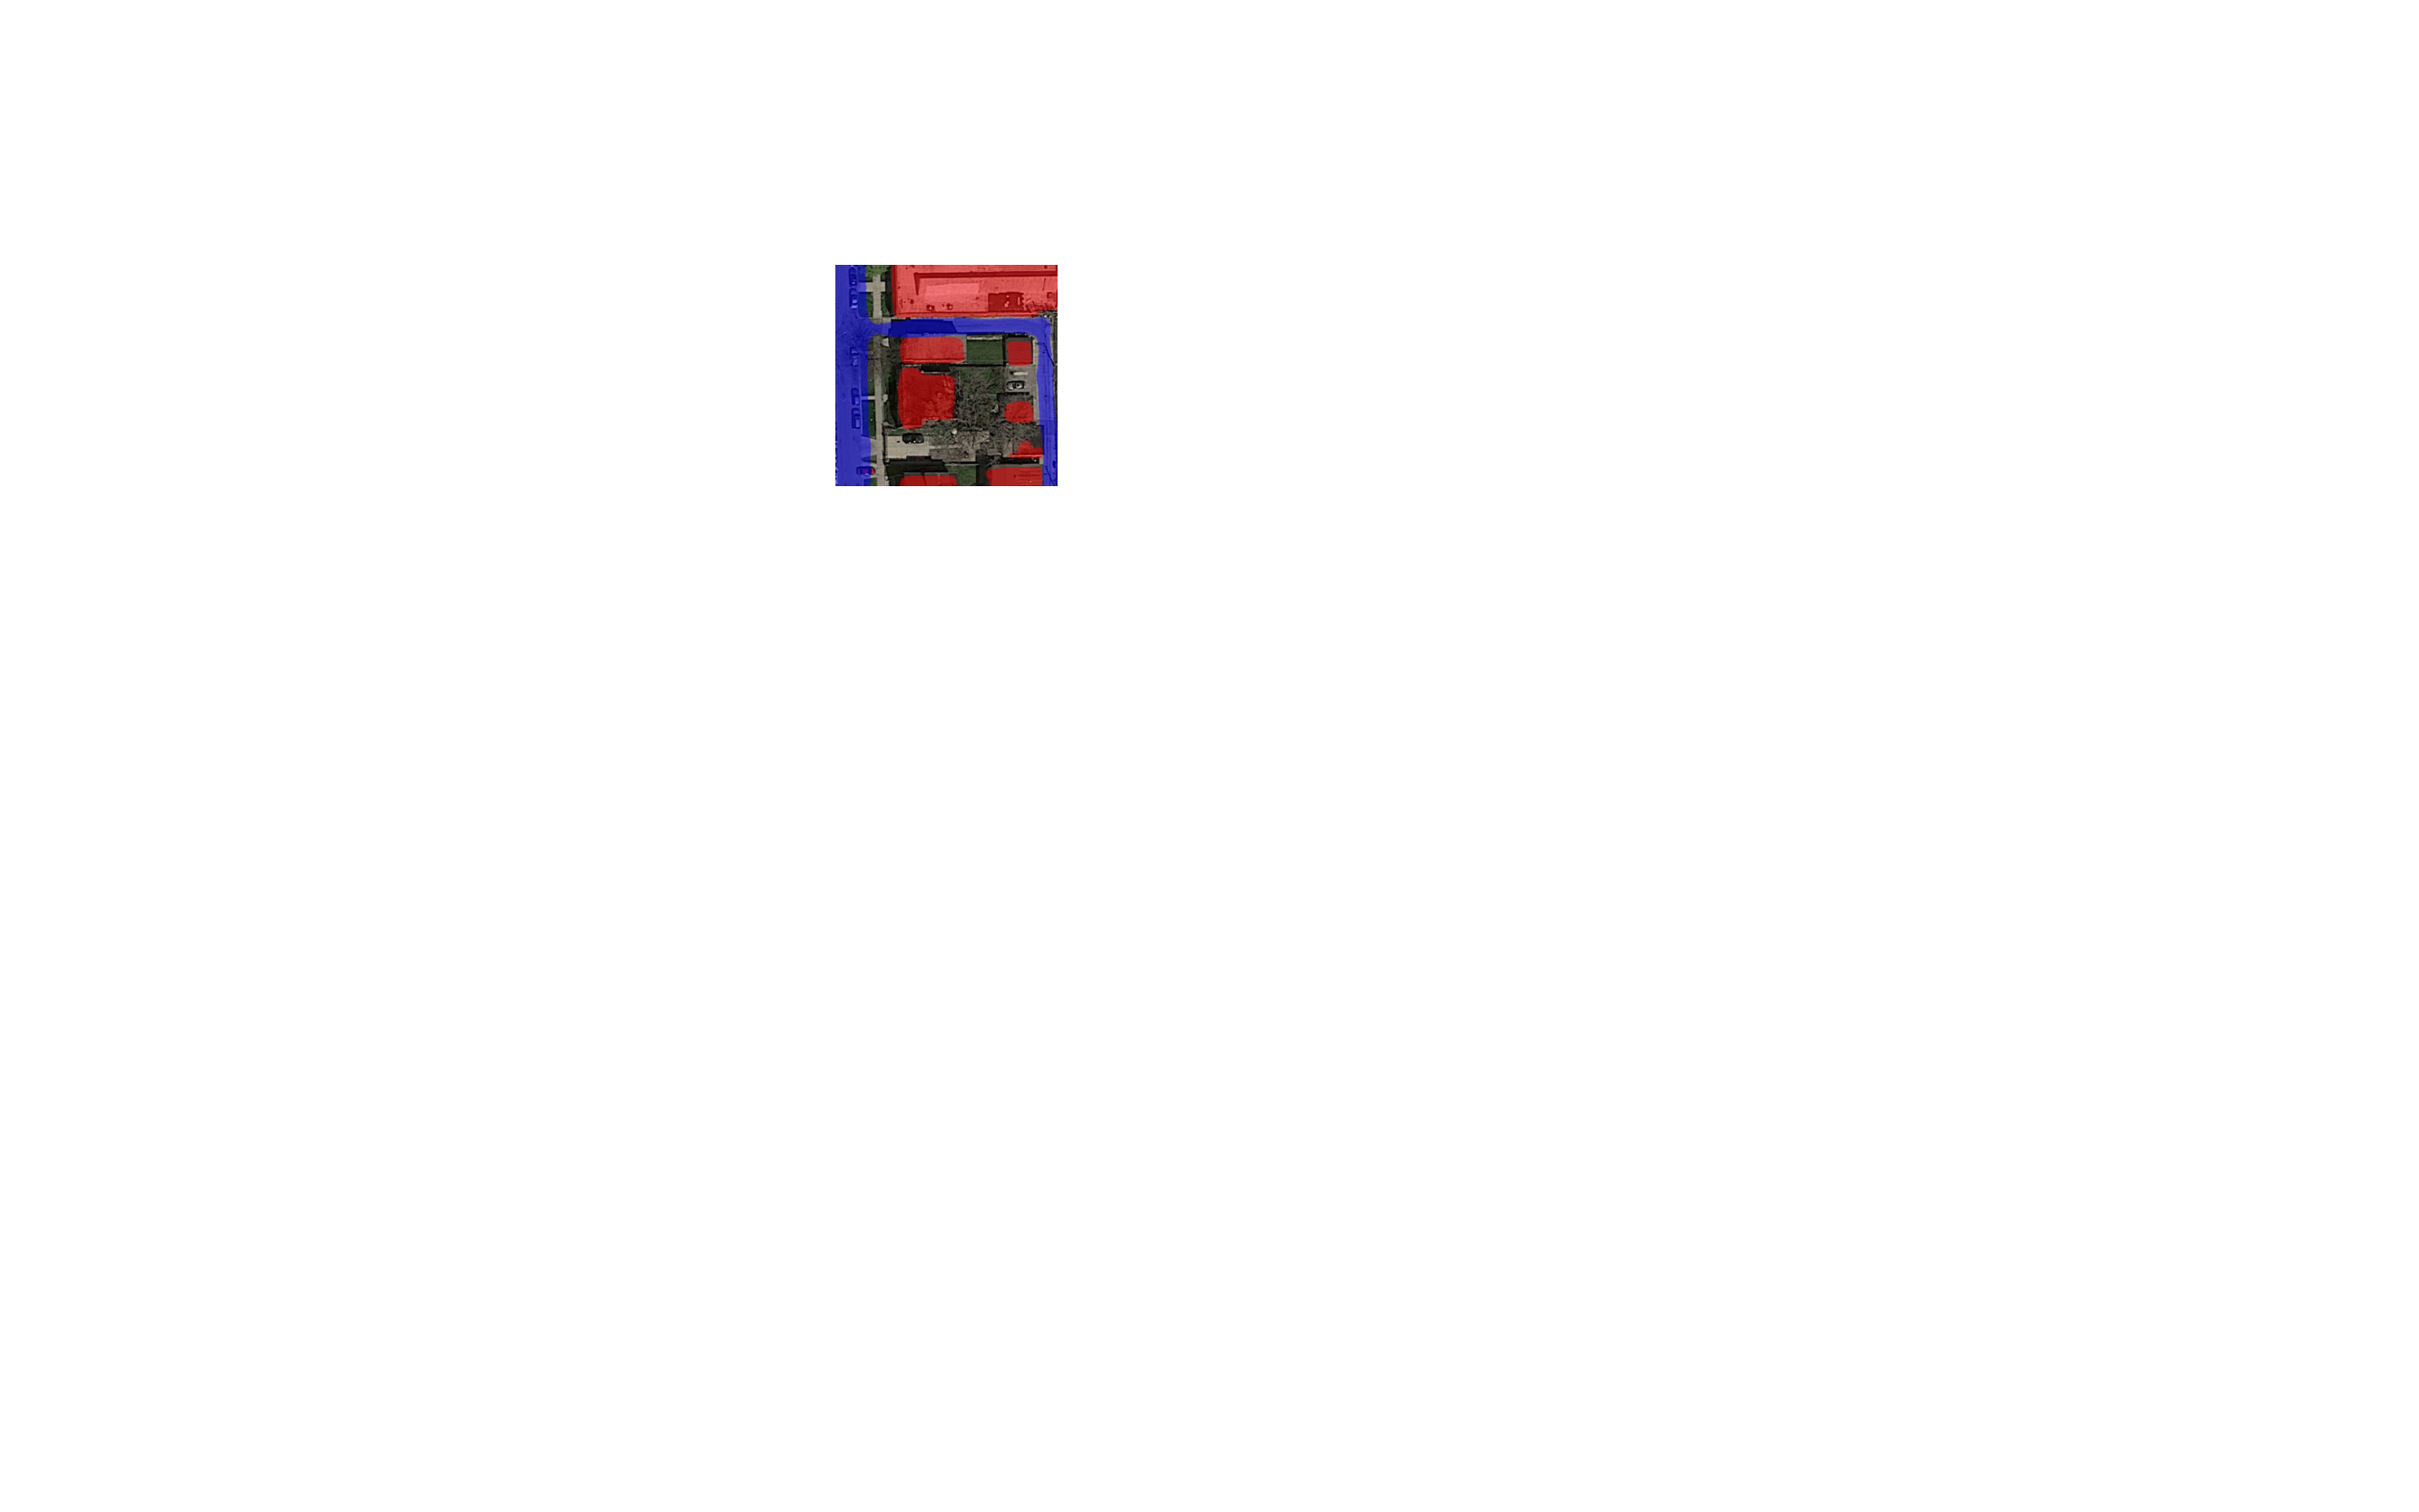
\includegraphics[width=\figfigfigfig\textwidth]{2-00-3.pdf}
	}
    \caption[Semantic segmentation in aerial images]{Semantic segmentation in aerial images. Image copyright owned by \cite{mspascal}. (a) and (c) are two aerial images. In the semantic segmentation result (b) and (d), the pixels covered by red color refer to buildings, while the pixels covered by blue color refer to roads.}
	\label{fig:mspascal}
\end{figure}

